\documentclass[a4paper,10pt,twoside]{article}

%===========PACOTES
\usepackage[body={170mm,235mm}]{geometry}
%\usepackage[portuguese]{babel}
\usepackage{a1}
\usepackage[english]{babel}
\usepackage[latin1]{inputenc} %permite o uso de acentos
%\usepackage[dvips]{color}
\usepackage{amsfonts,amssymb}
%\usepackage{epsfig}
\usepackage{amsmath}
\usepackage{graphicx}	

% makeidx
\usepackage{makeidx}
% make index
\makeindex
%\usepackage[pdftex]{graphicx}


\def\mapright#1#2#3{\smash{\mathop{\hbox to
#3{\rightarrowfill}}\limits^{#1}_{#2}}}

\def\mapleft#1#2#3{\smash{\mathop{\hbox to
#3{\leftarrowfill}}\limits^{#1}_{#2}}}

\def\mapright#1#2{\smash{\mathop{\hbox to 0.90cm{\rightarrowfill}}\limits^{#1}_{#2}}}
\def\mapleft#1#2{\smash{\mathop{\hbox to 0.90cm{\leftarrowfill}}\limits^{#1}_{#2}}}

\def\mapleftright#1#2{\smash{\mathop{\hbox to 0.80cm{\leftarrowfill \rightarrowfill}}\limits^{#1}_{#2}}}
\def\ext{\times \! \vrule depth0pt height5pt width0.35pt}

\def\H{\mathcal H}
\def\D{\mathcal D}
\def\B{\mathcal B}
\def\C{\mathbb C}
\def\R{\mathbb R}
\def\S{\mathbb S}
\def\U{\mathcal U}
\def\Z{\mathbb Z}

\title{Closed oriented 3-manifolds are equivalence classes of plane graphs
\footnote{2010 Mathematics Subject Classification: 
05C85 and 05C83 (primary), 57M27 and 57M15 (secondary)}} 
\author{S�stenes L. Lins}

\date{\today}


\begin{document}


\maketitle

\begin{abstract}
A {\em blink} is a plane graph with an arbitrary bipartition of its edges.
As a consequence of a recent result of Martelli, we show that the homeomorphisms classes
of closed oriented 3-manifolds are in 1-1 correspondence with classes of blinks. Two blinks
are equivalent if they are linked by a finite sequence of local moves, where each one
appears in a concrete list of 64 moves: they organize in 8 types,
each beeing essentlially the same move on 8 simply related configurations. 
The size of the list can be substantially
decreased at the cost of loosing symmetry, just by introducing a very simple move,
the ribbon move named $\beta_1$ (which is in principle redundant). Using  $\beta_1$
makes all the moves coming from plane duality (the starred moves), except for $\rho_2^\star$,
redundant.
\end{abstract}


\section{Statement of the Theorem}
This paper proves the following theorem:
\begin{theorem}
\label{theo:theorem}
 The classes homeomorphisms of closed oriented 3-maniflds are in 1-1 correspondence
 with the equivalence classes of blinks where two blinks are equivalent if they are
 linked by a finite sequence of the local moves where each term is 
 one of the 64 moves below\\
 \begin{center}
 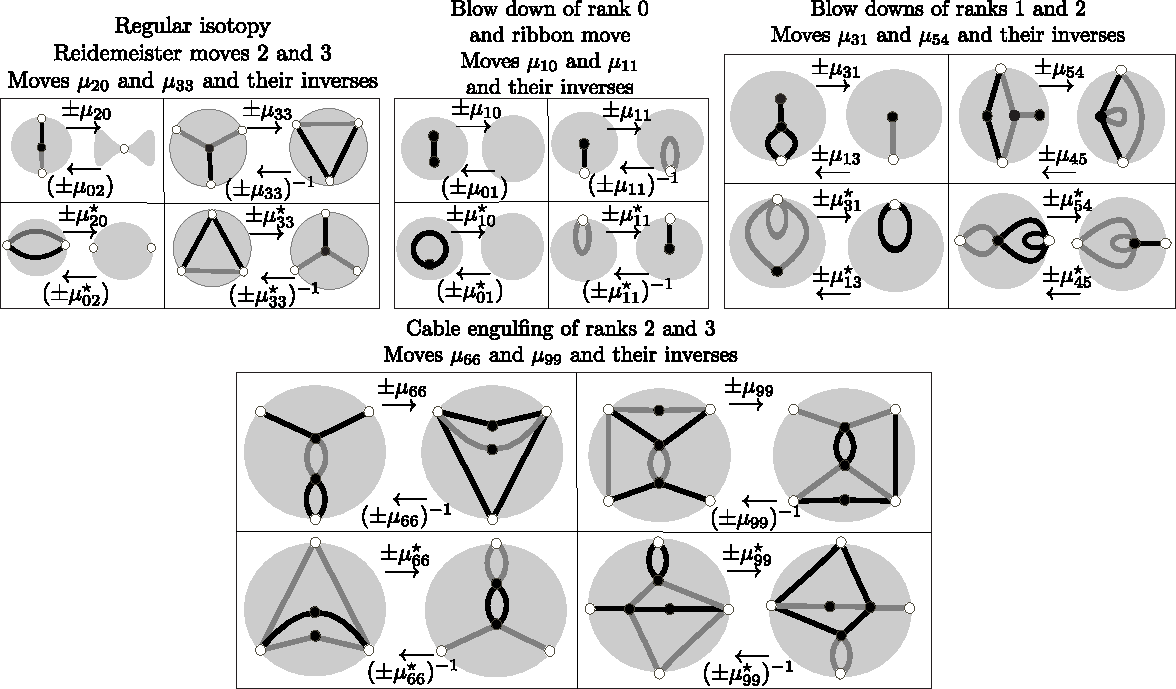
\includegraphics[width=16cm]{A.figs/blinkcalculus.pdf} 
  \end{center}
  \end{theorem}
 There are 64 local configurations divided into 32 pairs of left-right configurations,
 each one named a {\em coin}. A move replaces the left (right) coin of a pair by its right (left) 
 coin. The complementary sub-blink in the exterior a coin is completely arbitrary;
 its intersection with the corresponding internal coin is the set of 
 attachment vertices shown in the boundary of the disk (or pinched disk, in the case of $\rho_2$)
 where the coin lies. The number of such attachment vertices (one of 0,1,2,3,4) 
 is the subscript for the label of the move.

\section{Lickorish and moves by Kirby, Fenn-Rourke, Kauffman, Martelli}

A {\em knot} is an embedding of a circle, an $\mathbb{S}^1$, into $\mathbb{R}^3$ or  $\mathbb{S}^3$.
The {\em unknot} is a knot which is the boundary of a disk.
A {\em link with $k$ components} is an embedding of a disjoint union of $k$ copies of $\mathbb{S}^1$
into $\mathbb{R}^3$ or  $\mathbb{S}^3$. In this way, a knot is a link with one component.

Knots and links can be presented by their {\em decorated 
general position projections} into a fixed plane $\mathbb{R}^2$. {\em General position} means that 
in the image of the link there is no triple points and that at each neighborhood of
each double is the transversal crossing of two segments of the link, named {\em strands}. 
{\em Decorated} means that we keep the information
of which strand is the upper one, usually by removing a piece of the lower strand. In this paper
we use another way to decorate the link projections: the images of the link components are thich black curves
and the upper strands are indicated by a thinner white segment inside the thich black curve at the crossing.



In a grounding breaking work,  W.B.R. Lickorish in 1962, \cite{lickorish1962representation}, proved that
each closed orientable 3-manifold $\mathbb{M}^3$ can be encoded by a link in $\mathbb{S}^ 3$ 
where each one of its $k$ components
is endowed with an irreducible fraction (the framing) $\frac {\pm p}{q}$ 
where $q$ could be 0, and in the case $p$ must be 1 and the fraction
becomes $\pm \infty$. To construct $\mathbb{M}^3$ 
from the framed link we act as follows: after removing from $\mathbb{M}^3$
an $\epsilon$-neighborhood $(\mathbb{S}^ 1 \times \mathbb{D}^2)_i$ of the $i$-th link we are left with 
$\mathbb{M}^ 3\backslash \bigcup_{i=1}^k (\mathbb{S}^ 1 \times \mathbb{D}^2)_i=
\mathbb{S}^ 3\backslash \bigcup_{i=1}^k (\mathbb{S}^ 1 \times \mathbb{D}^2)_i$. The fraction specifies, in the 
toroidal boundary inside $\mathbb{S}^ 3$, the homology type $(\pm p,q)$ of the curve that
is contractible in the solid torus inside $\mathbb{M}^3$. For each component, we then
identify the simple curve given by the homological base pair with the meridian of a canonical copy of a 
solid torus in $\mathbb{R}^ 3$  so as to completely specify the pasting of the solid torus 
closing the toroidal hole.
Lickorish's breakthrough was to prove that any $\mathbb{M}^3$ has inside it a finite number
$k$ of disjoint solid tori so that $\mathbb{M}^ 3\backslash \bigcup_{i=1}^k 
(\mathbb{S}^ 1 \times \mathbb{D}^2)_i=
\mathbb{S}^ 3\backslash \bigcup_{i=1}^k (\mathbb{S}^1 \times \mathbb{D}^2)_i$.
Actually, this result had been proved 2 years before 
by A. H. Wallace \cite{wallace1960modifications} by using differential geometry. However
it was the purely topological flavor of Lickorish's proof that spurs the subsequent developments.
  
In 1978 R. Kirby published his, to become famous, calculus of framed links, \cite{kirby1978calculus}.
The gist of this paper is that two types of moves 
are enough to go from any framed
link inducing a closed oriented 3-manifold to any other such link inducing the same manifold.
One of the moves is absolutelly local: creating or cancellating a an unknot with frame in
$\{\infty,-\infty\}$. The other type of move, 
{\em the band move (\cite{kauffman1991knots}) (or handle sliding)} is non-local and infinite in number.


Shortly after in 1979 R. Fenn and C. Rourke (\cite{fenn1979kirby}) show that Kirby's moves could 
be replaced by an infinite number a single type of moves parametrized by $n$. This has been
a very useful reformulation with many applications, including Martelli's calculus (soon to be treated)
which uses it instead of the direct moves of Kirby. 

In the beginning of the 1990's L. Kauffman
presented (\cite{kauffman1991knots}) a completely plane diagramatic way to deal with the 
calculus of Kirby and of Fenn-Rourke. The basic idea comes from the fact that every 3-manifold is
induced by surgery on a framed link which has {\em only finite integer framings}, which D. Rolfsen call
{\em by honest surgery}, \cite{rolfsen2003knots}. The proof of this result uses that it is possible to
modify the framed link maintaining the induced 3-manifold so that every component becomes unknotted. 
A proof of this fact appears in Rolfsen's book. It also apears in page 137 of Kauffman-Lins monography,
\cite{kauffman1994tlr}. If a component is unknotted then 
it is simple to modify the link so that each component gets an integer framing, without 
distub the integrality of the framing of other components. So, without loss of
generality we may supose that all the components have finite integers as framings. Kauffman's proceeds
by adjusting each component by attaching to it a judicious number of curls so that the required framing of
a component coincides with the algebraic sum of its self-crossings. 
By specifying that the link is {\em blackboard framed}, we no longer need the framings.
In this work we only use blackboard framed links.

In an important recent paper B. Martelli \cite{martelli2012finite} presented a local finite reformulation of
the Fenn-Rourke version (\cite{fenn1979kirby}) of Kirby's calculus \cite{kirby1978calculus}. It remains
to be seen the consequences of Martelli' s result for obtaining new 3-manifold invariants.
Our objective here is to further reformulate Martelli's moves so as to obtain a calculus
of blinks, which is an exact combinatorial counterpart for factorizing homeomorphisms of
closed orientable 3-manifolds. This goal is desirable because it has the consequence that each 3-manifold
become a subtle class of plane graphs. Our exposition is complete and elementary seeking
to reach both audiences: topologists and combinatorialists. We feel that this result may be interesting
for Combinatorics as well as to Topology and may enhance both areas. Plane graphs are one of the most 
studied objects in mathematics. Some of their properties could be used in 3-manifolds and vice-versa. 
At any rate I am using here a recipe of Conway, \cite{hk}.


\begin{figure}[!h]
\begin{center}
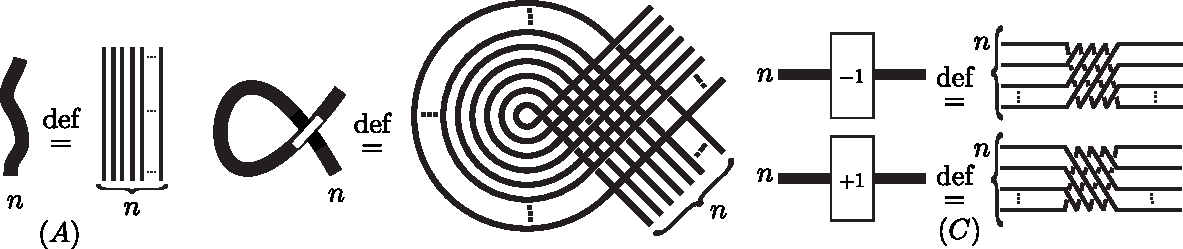
\includegraphics[width=16.5cm]{A.figs/somenotation.pdf} 
\caption{\sf Some notation}
\label{fig:somenotation}
\end{center}
\end{figure} 


\begin{figure}[!h]
\begin{center}
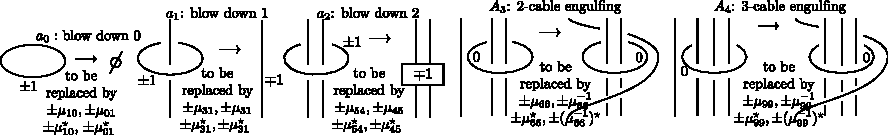
\includegraphics[width=16.5cm]{A.figs/Martelli.pdf} 
\caption{\sf Martelli's calculus on fractional framed links}
\label{fig:blinklinkgem}
\end{center}
\end{figure} 

\begin{figure}[!h]
\begin{center}
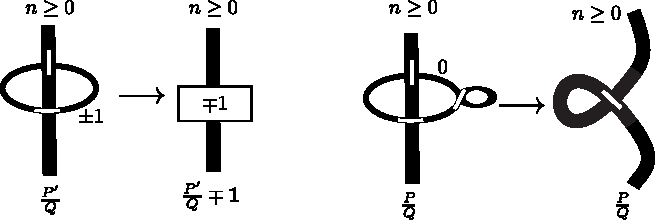
\includegraphics[width=13.5cm]{A.figs/FennRourkeAndKauffmanMove.pdf} 
\caption{\sf Fenn-Rourke infinite sequence of blown-down moves 
and their counterpart in Kauffman's blackboard framed links. These are
infinite sequence of local moves. Cases $n=0$ of these moves replace
an isolated $\pm 1$-framed component or the unknot with one crossing by nothing.
Martelli replaced the infinite sequence by the first three and two simple
moves which we call {\em 2- and 3- cable engulfing}, denoted by $A_3$ and $A_4$
shortly to be described. In our final form of the blink-coin calculus 
we use a revised versions of $A_3$ and $A_4$: the moves $a_3$ and $a_4$,
which seem substantially simpler to put on the blink-coin calculus}
\label{fig:FennRourkeAndKauffmanMove}
\end{center}
\end{figure} 


\section{Proof of the Theorem}

\begin{figure}[!h]
\begin{center}
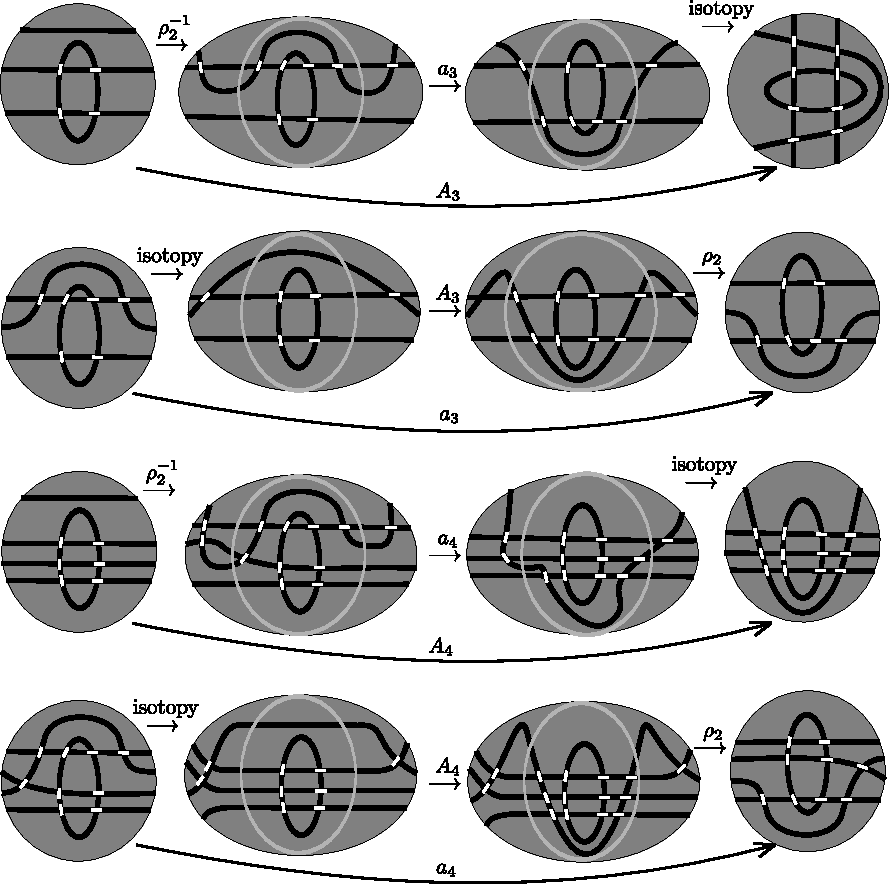
\includegraphics[width=14cm]{A.figs/proofequivalencea3A3a4A4.pdf} 
\caption{\sf A proof that in the presence of $\pm \rho_2^{\pm 1}$, $a_3 \equiv A_3$ and $a_4 \equiv A_4$ }
\label{fig:proofequivalencea3A3a4A4}
\end{center}
\end{figure} 
\begin{lemma}
 In the presence of  $\rho_2^{\pm 1}$, moves $\pm a_3$ and $\pm A_3$ are equivalent and so are
 $\pm a_4$ and $\pm A_4$.
\end{lemma}
\begin{proof}
 We refer to  Fig. \ref{fig:proofequivalencea3A3a4A4}. Its first line proves that $\pm a_3 \Rightarrow \pm A_3$.
 The second line proves that $\pm A_3 \Rightarrow \pm a_3$. The third line proves 
 that $\pm a_4 \Rightarrow \pm A_a$. The last line proves that $\pm A_4 \Rightarrow \pm a_4$. 
\end{proof}



\begin{figure}[!htb]
\begin{center}
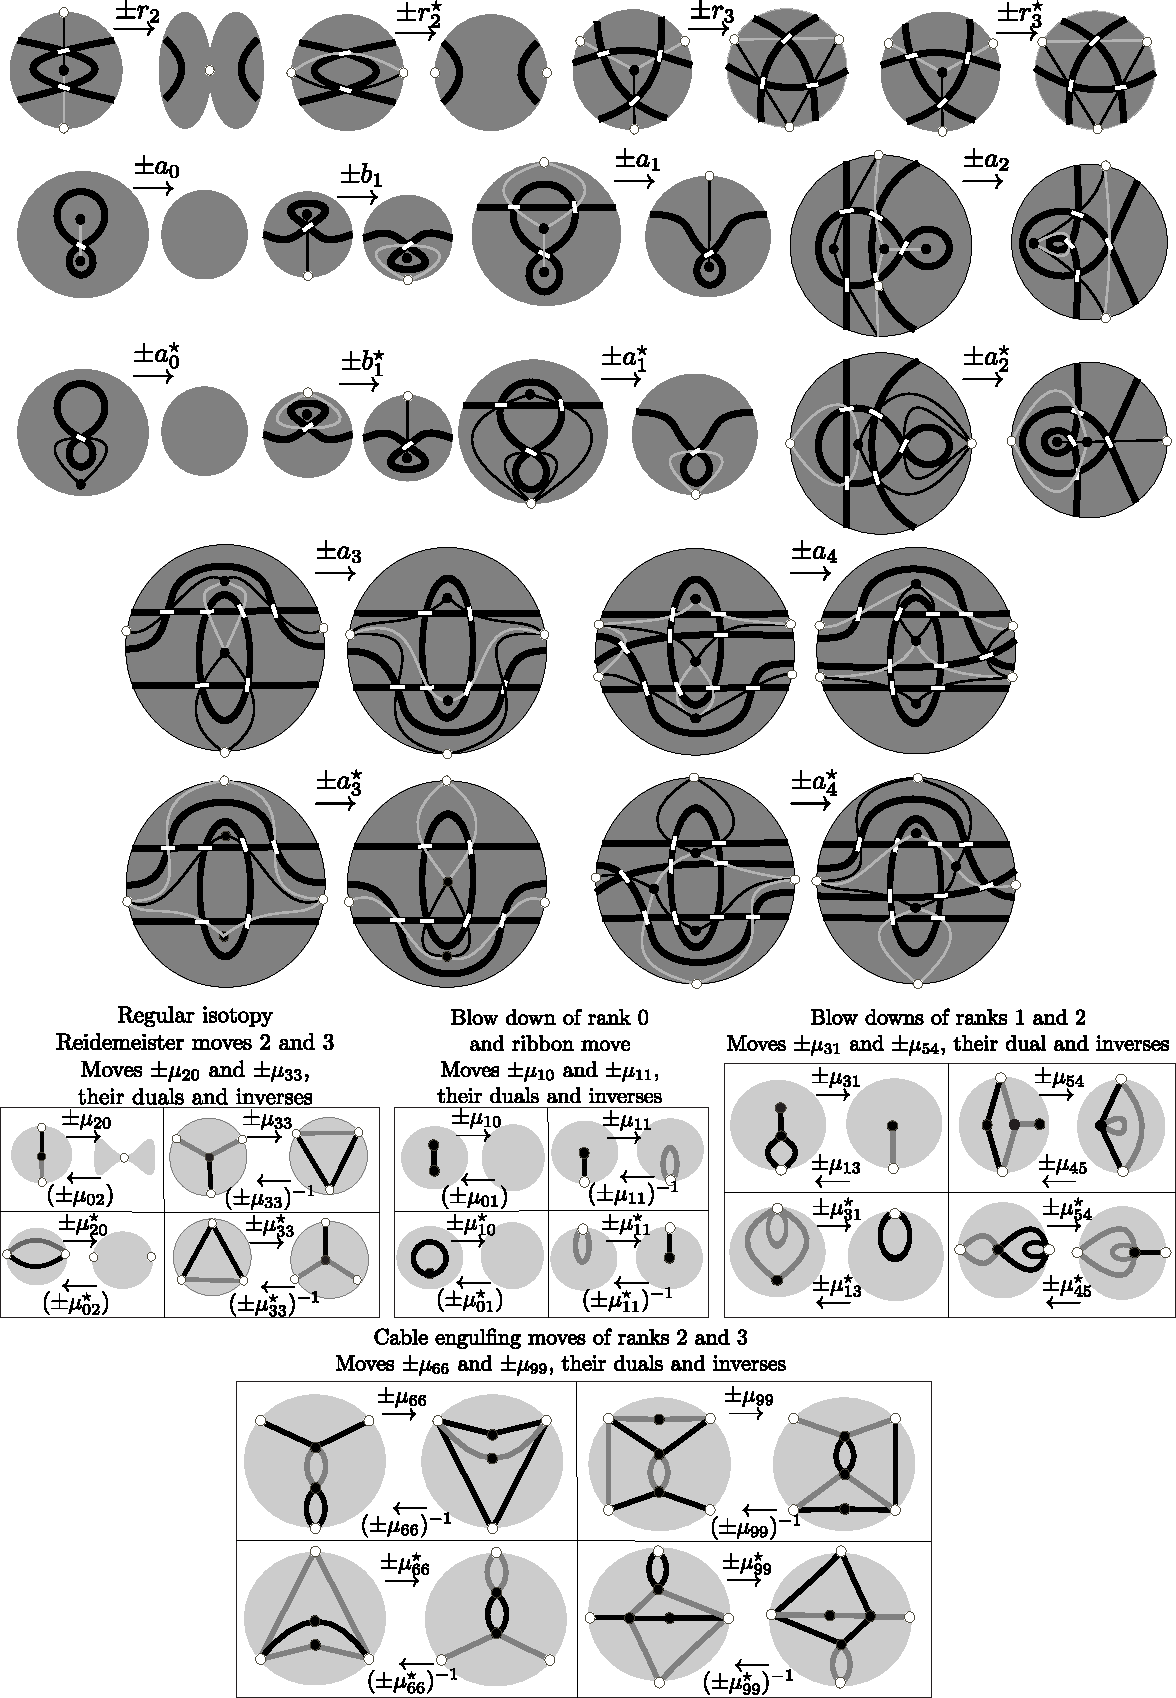
\includegraphics[scale=0.8]{A.figs/blinkandlinktogether.pdf}
\caption{Links \& blinks together implying moves for the blink calculus, concluding the proof of the Theorem 1.1}
\label{fig:blinkandlinktogether}
\end{center}
\end{figure}


% \begin{figure}[!h]
% \begin{center}
% \includegraphics[width=12.5cm]{A.figs/seconddoubtB.pdf}
% \caption{\sf Finding presentations for the fundamental groups of $M^ 3[2125]$ and $M^ 3[2165]$}
% \label{fig:seconddoubtB}
% \end{center}
% \end{figure}

%-----------------------------------
\bibliographystyle{plain}
%\bibliographystyle{is-alpha}
%\addcontentsline{toc}{bibliografia}{\MakeTextUppercase{Refer�ncias Bibliogr�ficas}}
%\bibliography{d:/slsl\3.DadosSostenes.35.ArtigosLivros.bibtexGoogleScholar/bibtexIndex.bib} % bib file is slsl.bib
%\bibliography{~/home/ricardo/Dropbox/35.ArtigosLivros.bibtexGoogleScholar/bibtexIndex.bib}
\bibliography{bibtexIndex.bib}
%\bibliography{slsl}


\vspace{5mm}
\begin{center}
\hspace{7mm}
\begin{tabular}{l}
   S\'ostenes L. Lins\\
   Centro de Inform\'atica, UFPE \\
   Av. Jornalista Anibal Fernandes s/n\\
   Recife, PE 50740-560 \\
   Brazil\\
   sostenes@cin.ufpe.br
\end{tabular}


\end{center}


\end{document}

\begin{figure}[!htb]
\begin{center}
\includegraphics[scale=0.8]{A.figs/seconddoubt.pdf}
\caption{Are these 3-manifolds homeomorphic?}
\label{fig:seconddoubt}
\end{center}
\end{figure}

% \printindex
